\documentclass{article}
\usepackage{arxiv}

\usepackage[utf8]{inputenc}
\usepackage[english, russian]{babel}
\usepackage[T2A, T1]{fontenc}
\usepackage{url}
\usepackage{booktabs}
\usepackage{amsfonts}
\usepackage{amsthm}
\usepackage{amssymb}
\usepackage{amsmath}
\usepackage{nicefrac}
\usepackage{microtype}
\usepackage{graphicx}
\usepackage{natbib}
\usepackage{doi}
\usepackage{algorithm}
\usepackage{algorithmic}

\newtheorem{theorem}{Theorem}
\newtheorem*{theorem-non}{Theorem}
\newtheorem{lemma}{Lemma}
\newtheorem*{lemma-non}{Lemma}
\newtheorem{assumption}{A}
\newtheorem*{assumption-non}{A}
%\newtheorem*{proof}{Proof}

\newcommand{\R}{\mathbb{R}}
\newcommand{\bb}{\mathbf{b}}
\newcommand{\bx}{\mathbf{x}}
\newcommand{\bA}{\mathbf{A}}


\title{Ускоренные методы нулевого порядка в гладкой выпуклой стохастической оптимизации}

\author{
	Хафизов Фанис \\
	\texttt{khafizov.fa@phystech.edu} \\
	%% examples of more authors
	\And
	Богданов Александр \\
	\texttt{bogdanov.ai@phystech.edu} \\
	\And
	Безносиков Александр \\
	\texttt{beznosikov.an@phystech.edu}
}
\date{}

\renewcommand{\shorttitle}{Ускоренные методы нулевого порядка}
\renewcommand{\undertitle}{}
%%% Add PDF metadata to help others organize their library
%%% Once the PDF is generated, you can check the metadata with
%%% $ pdfinfo template.pdf
\hypersetup{
pdftitle={Ускоренные методы нулевого порядка в гладкой выпуклой стохастической оптимизации},
pdfsubject={Стохастическая оптимизация},
pdfauthor={Хафизов Ф.А., Богданов А.И., Безносиков А.Н.},
pdfkeywords={Методы нулевого порядка},
}

\begin{document}
\maketitle

\begin{abstract}
Данная работа посвящена задачи оптимизации без доступа к градиенту целевой функции $f(x)$, из-за чего нам надо как-то его оценивать. Рассматривается безградиентный метод JAGUAR, использующий информацию о предыдущих вызовах и требует $\mathcal{O}(1)$ оракульных вызовов. Мы применяем эту аппроксимацию в ускоренном методе градиентного спуска и докажем его сходимость для выпуклой задачи оптимизации. Также сравним метод JAGUAR с другими известными способами на экспериментах.

\end{abstract}

\keywords{методы нулевого порядка, стохастическая оптимизация}

\section{Введение}
\subsection{Мотивация}
Стохастические градиентные методы являются необходимыми в решении различных оптимизационных задач. Однако в нынешних проблемах машинного обучения возникает потребность оценивать градиент, ввиду, например, дороговизны его подсчета, либо же незнания явного вида минимизируемой функции. Тогда на помощь приходят методы нулевого порядка. Так как имеется доступ только к значениям целевой функции $f$ в различных точках $x \in \R^d$, то необходимо строить методы, аппроксимирующие градиент, используя конечные суммы значений целевой функции.\\
Одним из возможных усложнений задачи является добавление шума к оракулу: вместо $f(x)$ он будет возвращать $f(x) + \delta (x)$. Более того, виды шума разделяются на стохастический \cite{lucchi2022theoretical} или детерминированный \cite{lobanov2023zeroorder}.\\
Другую важную роль в решении оптимизационных задач играют ускоренные методы. Они как правило имеют более быструю сходимость по сравнению со стандартными алгоритмами. Предложенный Нестеровым \cite{Nesterov1983AMF} быстрый градиентный метод является классическим примером.
\subsection{Смежные работы}
Впервые метод JAGUAR аппроксимации градиента был предложен в \cite{bogdanov2024aspects}, доказана сходимость для методов Франка-Вульфа и градиентного спуска для невыпуклой, выпуклой, и сильно-выпуклой задач. Также есть модификация алгоритма Франка-Вульфа для стохастического случая (рассмотрены случаи one-point feedback и two-point feedback).\\
В работе \cite{beznosikov2023order} рассмотрены ускоренные методы первого порядка в невыпуклых и сильно выпуклых задачах оптимизации, содержащих марковский шум. Там при аппроксимации градиента использовался рандомизированный размер батча. Результаты и подходы оттуда адаптированы под метод JAGUAR в данной работе.\\
State-of-the-art решения в области безградиентной оптимизации собраны в \cite{gasnikov2024randomized}. Представлены рандомизированные методы нулевого порядка, однако лишь для нестохастического случая.\\
Ускоренный безградиентный метод в гладкой выпуклой стохастической оптимизации был предложен в \cite{gorbunov2020accelerated}, но лишь в случае two-point feedback, который далеко не всегда реализуется на практике.
\subsection{Предложения}
Предлагается ускоренный метод, в качестве аппроксимации градиента использующий JAGUAR. Для него получены теоремы о скорости сходимости при разных ограничениях на целевую функцию (выпуклая, сильно-выпуклая, невыпуклая). Теоретическая часть подкреплена численным экспериментом: классификация на датасете небольшого размера и минимизация квадратичной функции. Проведено сравнение с методами $l_2$-smoothing и полной аппроксимацией градиента.


\section{Постановка задачи}
Как уже было упомянуто, задача подразделяется на детерминированный случай, когда $f_\delta$ зависит только от $x$, и стохастический, в котором есть зависимость от случайного вектора $\xi \sim \pi$.
\subsection{Детерминированный случай}
В этом разделе рассматривается детерминированная задача оптимизации:
\begin{equation}
 \min\limits_{x \in \R^d} f(x).
 \label{determenistic_problem}
\end{equation}
Мы полагаем, что есть доступ только к оракулу нулевого порядка, то есть, мы можем получать только значения $f(x)$, но не градиента $\nabla f(x)$. Следовательно, нужно как-то аппроксимировать градиент $\nabla f(x)$. Также предполагается, что оракул возвращает
\begin{equation}
 f_\delta (x) = f(x) + \delta (x).
\end{equation}
Для аппроксимации градиента используется следующая разностная схема:
\begin{equation}
\widetilde{\nabla}_i f_\delta (x) := \frac{f_\delta (x + \tau e_i) - f_\delta (x - \tau e_i)}{2\tau} e_i,
\label{diff_scheme}
\end{equation}
где $e_i$ --- вектор из стандартного базиса в $\R^d$, $\tau > 0$ --- достаточно мало.

\subsection{Стохастический случай}
В этом же разделе рассматривается более общая стохастическая задача:
\begin{equation}
 \min\limits_{x \in \R^d} f(x) := \mathsf{E}_{\xi \sim \pi}[f(x, \xi)],
\end{equation}
где $\xi$ --- случайный вектор из неизвестного распределения $\pi$. Здесь мы так же считаем, что у нас нет доступа к градиенту $\nabla f(x, \xi)$, а оракул нулевого порядка возвращает зашумленное значение функции $f_\delta (x, \xi) := f(x, \xi) + \delta (x, \xi)$.\\
Разделяются два вида аппроксимации градиента в стохастическом случае:
\begin{itemize}
 \item Two-point feedback (TPF)
 \begin{equation}
  \widetilde{\nabla}_i f_\delta (x, \xi) := \frac{f_\delta (x + \tau e_i, \xi) - f_\delta (x - \tau e_i, \xi)}{2\tau} e_i,
 \end{equation}
 \item One-point feedback (OPF)
 \begin{equation}
  \widetilde{\nabla}_i f_\delta (x, \xi^+, \xi^-) := \frac{f_\delta (x + \tau e_i, \xi^+) - f_\delta (x - \tau e_i, \xi^-)}{2\tau} e_i,
 \end{equation}
\end{itemize}
где $\xi, \xi^+, \xi^- \sim \pi$, $e_i$ --- базисный вектор в $R^d$, $\tau > 0$ --- достаточно мало.\\
В случае TPF в обоих точках, где мы вызываем оракула, одно и то же значение $\xi$, что может быть тяжело реализуемо. Также TPF является частным случаем OPF ($\xi^+ = \xi^- = \xi$).

\section{Основные результаты}
Для доказательств сходимости нам требуется сделать несколько предположений о функции $f$ и об оракуле $f_\delta$.
\subsection{Предположения}
\begin{assumption}[Гладкость]\label{A1}
 Функция $f$ является $L$-гладкой на $\R^d$ с константой $L > 0$, т.е.:
 \begin{equation}
  \exists L > 0: \forall x, y \in \R^d \hookrightarrow \|\nabla f(x) - \nabla f(y)\| \leqslant L \|x - y\|.
  \label{l_smoothness}
 \end{equation}
\end{assumption}

\begin{assumption}[Сильная выпуклость]\label{A2}
 Функция $f$ является $ \mu$-сильно выпуклой на $\R^d$, т.е.:
 \begin{equation}
  \exists \mu > 0: \forall x, y \in \R^d \hookrightarrow \frac{\mu}{2}\|x - y\|^2 \leqslant f(x) - f(y) - \langle \nabla f(y), x - y \rangle.
  \label{mu_strongly_convexity}
 \end{equation}
\end{assumption}


\begin{assumption}[Ограниченность оракульного шума]\label{A3}
 Оракульный шум ограничен некоторой константой $\Delta > 0$, т.е.:
 \begin{equation}
  \exists \Delta > 0: \forall x \in \R^d \hookrightarrow |\delta(x)| \leqslant \Delta.
  \label{bounded_oracle_noise}
 \end{equation}
\end{assumption}


\subsection{Алгоритм}
Предлагается следующая версия ускоренного градиентного метода с аппроксимацией вида (\ref{diff_scheme}), взятой по случайной координате.
\begin{algorithm}[!ht]
\caption{ Accelerated Gradient Descent }\label{agd_algorithm}
\begin{algorithmic}[1]
   \REQUIRE stepsize $\gamma > 0$, momentums $\theta, \eta, \beta, p$, number of iterations $N$, approximation parameter $\tau > 0$.
   \textbf{Initialization:} choose $x^0 = x_f^0$
   \FOR{$k=0, 1,  \ldots, N-1$}
		\STATE $x_g^k = \theta x_f^k + (1 - \theta)x^k$
		\STATE Sample $i \sim U\{1, \dots, d\}$
		\STATE $g^k = d\frac{f_\delta(x_g^k + \tau e_i) - f_\delta(x_g^k - \tau e_i)}{2\tau}e_i$
		\STATE $x_f^{k + 1} = x_g^k - p \gamma g^k$
		\STATE $x^{k + 1} = \eta x_f^{k + 1} + (p - \eta) x_f^k + (1 - p)(1 - \beta) x^k + (1 - p)\beta x_g^k$
   \ENDFOR
\end{algorithmic}
\end{algorithm}

При доказательстве сходимости понадобится следующая лемма.
\begin{lemma}\label{lemma1}
 Предположим A \ref{A1}, A \ref{A3}. Тогда для аппроксимации градиента $g^k$ в алгоритме \ref{agd_algorithm} выполняется
 \begin{equation}
  \|\nabla f(x_g^k) - \mathbb{E}g^k\|^2 \leqslant d \left(\frac{L\tau}{2} + \frac{\Delta}{\tau}\right)^2.
  \label{norm_of_expectation}
 \end{equation}
 \begin{equation}
  \mathbb{E}[\|\nabla f(x_g^k) - g^k\|^2] \leqslant 2d \|\nabla f(x_g^k)\|^2 + 2 d^2 \left(\frac{L\tau}{2} + \frac{\Delta}{\tau}\right)^2.
  \label{expectation_of_norm}
 \end{equation}
\end{lemma}

Сформулируем теорему о сходимости метода на описанном классе функций.

\begin{theorem}[Сходимость (\ref{agd_algorithm}) в случае детерминированного шума]\label{theorem1}
  Предположим A \ref{A1} - A \ref{A3}. Тогда ускоренный градиентный спуск (Algorithm \ref{agd_algorithm}) имеет скорость сходимости на задаче (\ref{determenistic_problem}):
  \begin{equation}
   \begin{aligned}
   \mathbb{E}\left[\|x^N - x^*\|^2 + \frac{6}{\mu} (f(x_f^N) - f(x^*))\right] \leqslant \exp\left(- N\sqrt{\frac{p^2\mu\gamma}{3}}\right) \left(\|x^0 - x^*\|^2 + \frac{6}{\mu} (f(x_f^0) - f(x^*))\right) +\\ +\frac{3 \sqrt{3\gamma}}{\mu^{3/2}} \cdot d \left(\frac{L\tau}{2} + \frac{\Delta}{\tau}\right)^2\left(2 + \sqrt{\frac{3}{\gamma\mu}}\right),
   \label{deterministic_convergence}
   \end{aligned}
  \end{equation}
  где $\gamma \in (0, \frac{3}{4L}], \beta, \theta, \eta, p$ такие, что:

  \begin{equation}
   p \simeq (2(1 + \gamma L))^{-1}, \beta \simeq \sqrt{p^2 \mu \gamma}, \eta \simeq \sqrt{\frac{1}{\mu\gamma}}, \theta \simeq \frac{p \eta^{-1} - 1}{\beta p \eta^{-1} - 1.}
  \end{equation}

\end{theorem}

\section{Вычислительный эксперимент}
В эксперименте рассматриваются две задачи: минимизация квадратичной функции и логистическая регрессия на датасете mushrooms. Ускоренный градиентный спуск сравнивается со стандартным градиентным спуском и с методом Нестерова. В качестве аппроксимации градиента используется разностная схема (\ref{diff_scheme}), взятая по каждому базисному вектору $e_i, i = \overline{1, d}$.\\
В ходе последующих экспериментов рассматривался детерминированный шум в виде округления до 6 знаков после запятой (шум ограничен $10^{-6}$ по абсолютной величине), и параметр $\tau = 10^{-5}$.
\subsection{Квадратичная задача}
В качестве целевой функции выступает
\begin{equation}
 f(x) = x^T A x - b^T x + c,
\end{equation}
где $A \in \mathbb{S}_d$ --- случайная симметричная матрица с собственными значениями на отрезке $[\mu, L]$, $b \in \R^d, c \in \R$ --- случайные.\\
Все методы запускаются из одной и той же случайной точки $x^0 \in \R^d$.
Сходимость рассматриваем по аргументу целевой функции $\frac{\|x^k - x^*\|}{\|x^0 - x^*\|}(\textnormal{OracleCalls}(k))$, где $x^k$ --- значение аргумента на $k$-й итерации, $x^*$ --- точка оптимума, найденная численно, $x^0$ --- стартовая точка алгоритма, $\textnormal{OracleCalls}(k)$ --- суммарное количество вызовов оракула за $k$ итераций.
\begin{figure}[!htbp]
\centering
  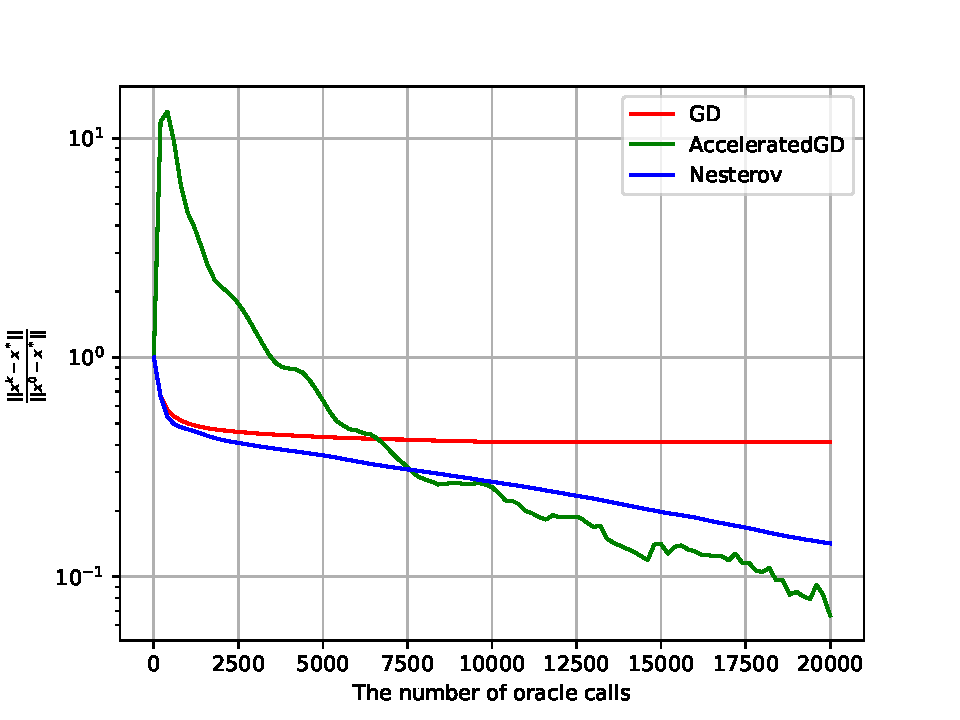
\includegraphics[width=0.7\textwidth]{../figures/Deterministic_quadratic_GD_AGD_Nesterov_15.pdf}
 \caption{Зависимость относительной ошибки $\frac{\|x^k - x^*\|}{\|x^0 - x^*\|}$ от числа оракульных вызовов для методов градиентного спуска, ускоренного градиентного спуска и Нестерова на квадратичной задаче минимизации}
  \label{fig:non-stochastic_logreg}
\end{figure}

\subsection{Логистическая регрессия}
Оптимизируется модель логистической регрессии с $L_2$-регуляризацией вида
\begin{equation}
 \min\limits{w \in R^d} f(w) = \frac{1}{m}\sum\limits_{k = 1}^m \log(1 + \exp(-y_k \cdot (Xw)_k)) + \lambda \|w\|_2^2,
\end{equation}
где взято $\lambda = 0,1$.\\
В логистической регрессии используется датасет mushrooms из библиотеки LibSVM. В качестве осей графика применяются $\|\nabla f(x^k)\| (\textnormal{OracleCalls}(k))$.
\begin{figure}[!htbp]
\centering
  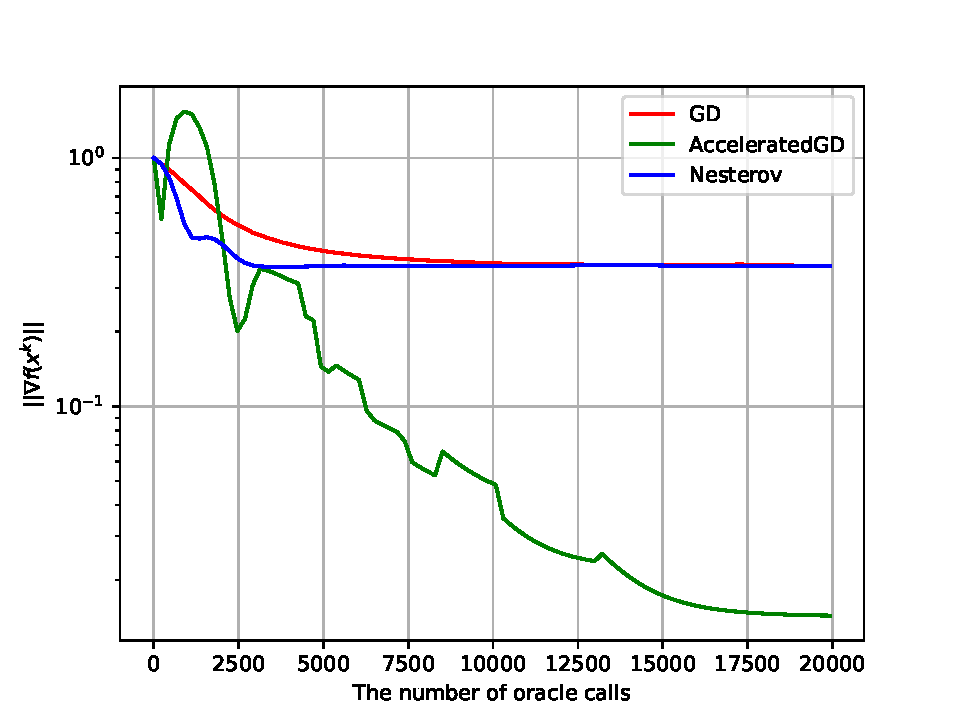
\includegraphics[width=0.7\textwidth]{../figures/Non_stochastic_Logreg_GD_AGD_Nesterov_15_1e-07_1e-05.pdf}
 \caption{Зависимость относительной ошибки $\|\nabla f(x^k)\|$ от числа оракульных вызовов для методов градиентного спуска, ускоренного градиентного спуска и Нестерова на задаче логистической регрессии}
  \label{fig:non-stochastic_logreg}
\end{figure}
\subsection{Предварительный отчет}
В проведенных экспериментах ускоренный метод показал себя лучше других, хотя, например, в квадратичной задаче поначалу он ведет себя намного хуже. В задаче логистической регрессии предложенный метод сильно обходит остальные методы.
\section{Анализ ошибки}
Посмотрим, как величина $\tau$ влияет на сходимость. С одной стороны, чем она меньше, тем более близкие точки мы берем, тем лучше линейная аппроксимации приближает функцию на этом отрезке, тем точнее должна быть оценка градиента. С другой стороны, присутствует детерминированный шум и слишком близкие точки будут давать большую погрешность. Для сравнения также построим график для метода с градиентом, вычисленным аналитически, считая стоимость вычисления градиента за $d$ оракульных вызовов. Он моделирует идеальные условия, когда $\Delta = 0, \tau \to 0$.
\subsection{Квадратичная задача}
Все описанные в секции вычислительного эксперимента параметры сохранены, за исключением переменного $\tau$.\\
\begin{figure}[!htbp]
\centering
  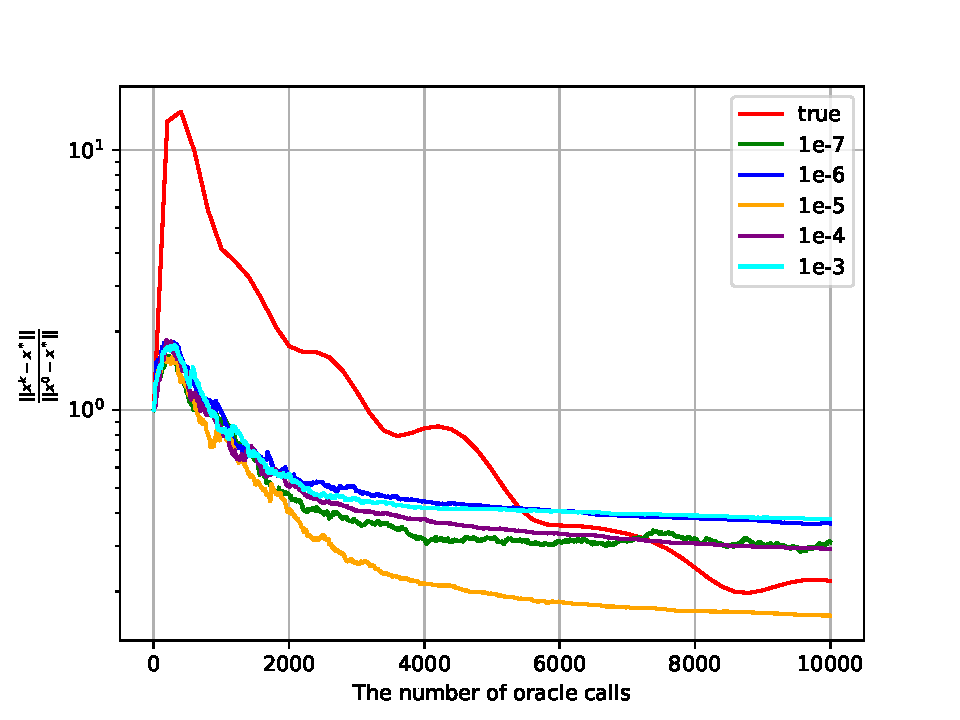
\includegraphics[width=0.7\textwidth]{../figures/Error_analysis_quadratic_sigma=1e-6.pdf}
 \caption{Зависимость относительной ошибки $\frac{\|x^k - x^*\|}{\|x^0 - x^*\|}$ от числа оракульных вызовов для Accelerated GD с изменяющимся значением $\tau$, а также Accelerated GD с аналитически вычисленным градиентом, квадратичная задача.}
  \label{fig:non-stochastic_quadratic}
\end{figure}
В построенном графике наблюдается, что параметр $\tau=10^{-3}$ является оптимальным из рассмотренных. Также видно, что методы, использующие аппроксимацию градиента на небольшом количестве итераций опережают версию с честным градиентом. Обясняется это тем, что последний делает много оракульных вызовов, как следствие мало шагов, и не успевает накопить моменты.
\subsection{Логистическая регрессия}
Условия также как в вычислительном эксперименте, за исключением изменений, описанных выше.
\begin{figure}[!htbp]
\centering
  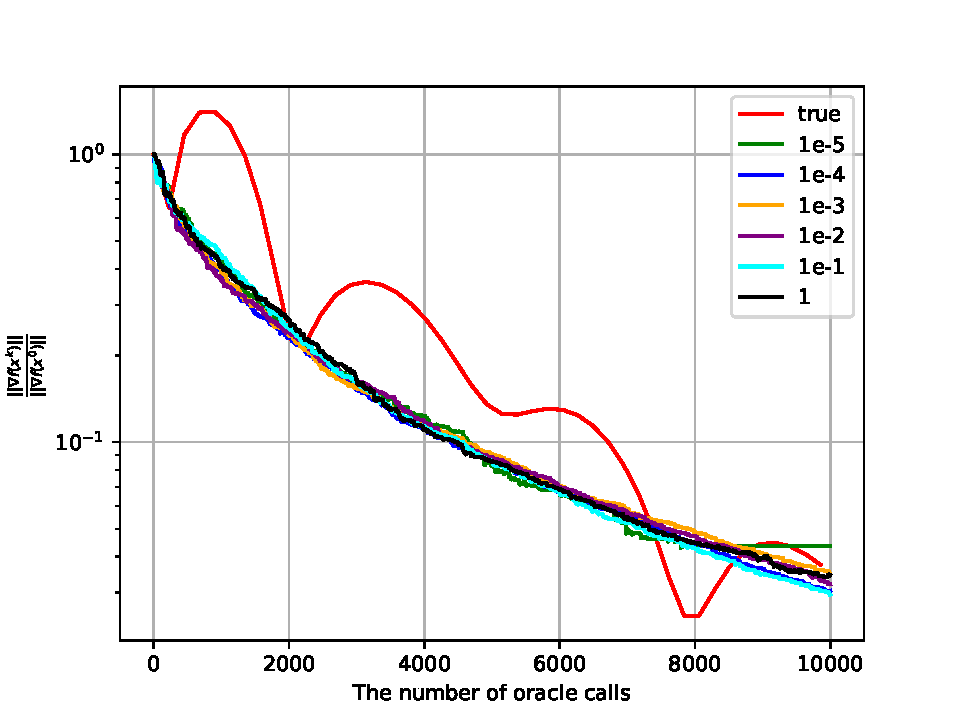
\includegraphics[width=0.7\textwidth]{../figures/Error_analysis_logreg_sigma=1e-6.pdf}
 \caption{Зависимость относительной ошибки $\frac{\|\nabla f(x^k)\|}{\|\nabla f(x^0)\|}$ от числа оракульных вызовов для Accelerated GD с изменяющимся значением $\tau$, а также Accelerated GD с аналитически вычисленным градиентом, логистическая регрессия.}
  \label{fig:non-stochastic_logreg}
\end{figure}
Здесь хорошо сходятся методы со значениями $\tau \in [10^{-4}, 10^{-1}]$. Также по сравнению с истинным градиентом, сходимость выглядит более стабильно.
\bibliographystyle{plain}
\bibliography{Khafizov2024AcceleratedZeroOrderMethods}

\newpage
\appendix
\begin{lemma}[Lemma \ref{lemma1}]\label{lemma1_appendix}
 Предположим A \ref{A1}, A \ref{A3}. Тогда для аппроксимации градиента $g^k$ в алгоритме \ref{agd_algorithm} выполняется
 \begin{equation}
  \|\nabla f(x_g^k) - \mathbb{E}g^k\|^2 \leqslant d \left(\frac{L\tau}{2} + \frac{\Delta}{\tau}\right)^2.
  \label{norm_of_expectation_appendix}
 \end{equation}
 \begin{equation}
  \mathbb{E}[\|\nabla f(x_g^k) - g^k\|^2] \leqslant 2d \|\nabla f(x_g^k)\|^2 + 2 d^2 \left(\frac{L\tau}{2} + \frac{\Delta}{\tau}\right)^2.
  \label{expectation_of_norm_appendix}
 \end{equation}
\end{lemma}
\begin{proof}
  $$\|\nabla f(x_g^k) - \mathbb{E} g^k\|^2 = \left|\left| \nabla f(x_g^k) - \mathbb{E}\left[d\frac{f(x_g^k + \tau e_i) - f(x_g^k - \tau e_i)}{2\tau} e_i + d\frac{\delta(x_g^k + \tau e_i) - \delta(x_g^k - \tau e_i)}{2\tau} e_i\right]\right|\right|^2 = $$
  $$=\sum\limits_{i = 1}^d \left|\frac{f(x + \tau e_i) - f(x - \tau e_i)}{2\tau} - \nabla_i f(x_g^k) - \frac{\delta(x + \tau e_i) - \delta(x - \tau e_i)}{2\tau}\right|^2 \leqslant$$
  $$\leqslant \sum\limits_{i = 1}^d\left( \left|\frac{1}{2\tau} \int\limits_{-\tau}^\tau \langle f(x_g^k + t e_i) - \nabla f(x_g^k), e_i \rangle dt\right| + \frac{\Delta}{\tau}\right)^2 \leqslant$$
  $$\leqslant \sum\limits_{i = 1}^d\left( \frac{1}{2\tau} \int\limits_{-\tau}^\tau \|f(x_g^k + t e_i) - \nabla f(x_g^k)\|_2 \cdot \|e_i\|_2 dt + \frac{\Delta}{\tau}\right)^2 \leqslant$$
  $$\leqslant \sum\limits_{i = 1}^d\left( \frac{1}{2\tau} \int\limits_{-\tau}^\tau L |t| dt + \frac{\Delta}{\tau}\right)^2 = \sum\limits_{i = 1}^d\left( \frac{L\tau}{2} + \frac{\Delta}{\tau} \right)^2 = d \left(\frac{L\tau}{2} + \frac{\Delta}{\tau}\right)^2.$$

  $$\mathbb{E}[\|\nabla f(x_g^k) - g^k\|^2] = \frac{1}{d} \sum\limits_{i = 1}^d \left|\left|\nabla f(x_g^k) - d \frac{f(x_g^k + \tau e_i) - f(x_g^k - \tau e_i)}{2\tau} e_i - d\frac{\delta(x_g^k + \tau e_i) - \delta(x_g^k - \tau e_i)}{2 \tau} e_i\right|\right|^2=$$
  $$=\frac{1}{d} \sum\limits_{i = 1}^d \left(\sum\limits_{j \neq i} |\nabla_j f(x_g^k)|^2 + \left|d\left(\frac{f(x_g^k + \tau e_i) - f(x_g^k - \tau e_i)}{2\tau} - \nabla_i f(x_g^k)\right) + (d - 1) \nabla_i f(x_g^k) + d \frac{\delta(x_g^k + \tau e_i) - \delta(x_g^k - \tau e_i)}{2 \tau}\right|^2\right) \leqslant$$
  $$\leqslant \frac{1}{d} \sum\limits_{i = 1}^d \left(\|\nabla f(x_g^k)\|^2 + \left(\left|\frac{d}{2\tau} \int\limits_{-\tau}^\tau \langle f(x_g^k + t e_i) - \nabla f(x_g^k), e_i \rangle dt\right| + (d - 1)|\nabla_i f(x_g^k)| + d \frac{\Delta}{\tau}\right)^2\right)\leqslant$$
  $$\leqslant \frac{1}{d} \sum\limits_{i = 1}^d \left(\|\nabla f(x_g^k)\|^2 + \left(d\frac{L\tau}{2} + (d - 1)|\nabla_i f(x_g^k)| + d \frac{\Delta}{\tau}\right)^2\right)\leqslant$$
  $$\leqslant \frac{1}{d} \sum\limits_{i = 1}^d \left(\|\nabla f(x_g^k)\|^2 + 2\left(d\frac{L\tau}{2} + d \frac{\Delta}{\tau}\right)^2 + 2(d - 1)^2|\nabla_i f(x_g^k)|^2\right)=$$
  $$=\|\nabla f(x_g^k)\|^2 + 2 d^2 \left(\frac{L\tau}{2} + \frac{\Delta}{\tau}\right)^2 + 2 \frac{(d - 1)^2}{d} \|\nabla f(x_g^k)\|^2 \leqslant 2d \|\nabla f(x_g^k)\|^2 + 2 d^2 \left(\frac{L\tau}{2} + \frac{\Delta}{\tau}\right)^2.$$
\end{proof}

\begin{lemma}(Неравенство из доказательства Theorem 6 в работе \cite{beznosikov2023order})
Предположим A \ref{A1} - A \ref{A3}. В Algoritm \ref{agd_algorithm} коэффициенты $\gamma \in (0, \frac{3}{4L}], \beta, \theta, \eta, p$ подобраны следующим образом:
\begin{equation}
  p \simeq (2(1 + \gamma L))^{-1}, \beta \simeq \sqrt{p^2 \mu \gamma}, \eta \simeq \sqrt{\frac{1}{\mu\gamma}}, \theta \simeq \frac{p \eta^{-1} - 1}{\beta p \eta^{-1} - 1.}
\end{equation}
Тогда справедливо неравенство:
$$\mathbb{E}[\|x^{k + 1} - x^*\|^2 + 2 \gamma \eta^2 (f(x_f^{k + 1}) - f(x^*))] \leqslant$$
$$\leqslant (1 - \beta / 2) \|x^k - x^*\|^2 + (1 - p/\eta) 2 \gamma \eta^2 (f(x_f^k) - f(x^*)) + p \eta^2 \gamma^2 (1 + 2p/\beta) \|\mathbb{E}[g^k] - \nabla f(x_g^k)\|^2 + $$
\begin{equation}
+2 p^2 \eta^2 \gamma^2 (1 + \gamma L) \mathbb{E}[\|g^k - \nabla f(x_g^k)\|^2] - p \gamma^2 \eta^2 (1 - 2p(1 + \gamma L))\|\nabla f(x_g^k)\|^2
\label{theorem_inequality}
\end{equation}
\end{lemma}

\begin{theorem}[Theorem \ref{theorem1}]\label{theorem1_appendix}
   Предположим A \ref{A1} - A \ref{A3}. Тогда ускоренный градиентный спуск (Algorithm \ref{agd_algorithm}) имеет скорость сходимости на задаче (\ref{determenistic_problem}):
  \begin{equation}
   \begin{aligned}
   \mathbb{E}\left[\|x^N - x^*\|^2 + \frac{6}{\mu} (f(x_f^N) - f(x^*))\right] \leqslant \exp\left(- N\sqrt{\frac{p^2\mu\gamma}{3}}\right) \left(\|x^0 - x^*\|^2 + \frac{6}{\mu} (f(x_f^0) - f(x^*))\right) +\\ +\frac{3 \sqrt{3\gamma}}{\mu^{3/2}} \cdot d \left(\frac{L\tau}{2} + \frac{\Delta}{\tau}\right)^2\left(2 + \sqrt{\frac{3}{\gamma\mu}}\right),
   \label{deterministic_convergence}
   \end{aligned}
  \end{equation}
  где $\gamma \in (0, \frac{3}{4L}], \beta, \theta, \eta, p$ такие, что:

  \begin{equation}
   p \simeq (2(1 + \gamma L))^{-1}, \beta \simeq \sqrt{p^2 \mu \gamma}, \eta \simeq \sqrt{\frac{1}{\mu\gamma}}, \theta \simeq \frac{p \eta^{-1} - 1}{\beta p \eta^{-1} - 1.}
  \end{equation}
\end{theorem}
\begin{proof}
Подставим (\ref{norm_of_expectation_appendix}) и (\ref{expectation_of_norm_appendix}) в (\ref{theorem_inequality}).
$$\mathbb{E}[\|x^{k + 1} - x^*\|^2 + 2 \gamma \eta^2 (f(x_f^{k + 1}) - f(x^*))] \leqslant (1 - \beta / 2) \|x^k - x^*\|^2 + (1 - p/\eta) 2 \gamma \eta^2 (f(x_f^k) - f(x^*)) +$$
$$ + p \eta^2 \gamma^2 (1 + 2p/\beta) \|\mathbb{E}[g^k] - \nabla f(x_g^k)\|^2 + 2 p^2 \eta^2 \gamma^2 (1 + \gamma L) \mathbb{E}[\|g^k - \nabla f(x_g^k)\|^2] - p \gamma^2 \eta^2 (1 - 2p(1 + \gamma L))\|\nabla f(x_g^k)\|^2 \leqslant$$

$$\leqslant (1 - \beta / 2) \|x^k - x^*\|^2 + (1 - p/\eta) 2 \gamma \eta^2 (f(x_f^k) - f(x^*)) + p \eta^2 \gamma^2 (1 + 2p/\beta) d \left(\frac{L\tau}{2} + \frac{\Delta}{\tau}\right)^2+$$
$$+ 2 p^2 \eta^2 \gamma^2 (1 + \gamma L) \left(2d \|\nabla f(x_g^k)\|^2 + 2 d^2 \left(\frac{L\tau}{2} + \frac{\Delta}{\tau}\right)^2\right) - p \gamma^2 \eta^2 (1 - 2p(1 + \gamma L))\|\nabla f(x_g^k)\|^2 =$$
$$=(1 - \beta / 2) \|x^k - x^*\|^2 + (1 - p/\eta) 2 \gamma \eta^2 (f(x_f^k) - f(x^*)) + $$
$$+ p \eta^2 \gamma^2 d\left(\frac{L\tau}{2} + \frac{\Delta}{\tau}\right)^2 \left(1 + 2p/\beta + 4pd(1 + \gamma L)\right)+$$
$$+p \gamma \eta^2 \|\nabla f(x_g^k)\|^2 (2p(1 + \gamma L) \cdot 2d + 2p(1 + \gamma L) - 1)$$

Возьмем $p = \frac{1}{2(1 + \gamma L)(2d + 1)}$.
$$\mathbb{E}[\|x^{k + 1} - x^*\|^2 + 2 \gamma \eta^2 (f(x_f^{k + 1}) - f(x^*))]\leqslant$$
$$\leqslant (1 - \beta / 2) \|x^k - x^*\|^2 + (1 - p/\eta) 2 \gamma \eta^2 (f(x_f^k) - f(x^*)) + p \eta^2 \gamma^2 d\left(\frac{L\tau}{2} + \frac{\Delta}{\tau}\right)^2 \left(1 + 2p/\beta + 4pd(1 + \gamma L)\right)$$
Теперь выберем $\beta/2 = p/\eta$, $p\eta\gamma = 3\beta/2\mu$.
$$\mathbb{E}[\|x^{k + 1} - x^*\|^2 + 2 \gamma \eta^2 (f(x_f^{k + 1}) - f(x^*))] \leqslant$$
$$\leqslant (1 - \beta / 2) \left(\|x^k - x^*\|^2 + 2 \gamma \eta^2 (f(x_f^k) - f(x^*))\right) + \frac{9\beta^2}{4\mu^2} \cdot 2(1 + \gamma L) (2d + 1) d \left(\frac{L\tau}{2} + \frac{\Delta}{\tau}\right)^2\left(1 + 2p/\beta + 4pd(1 + \gamma L)\right) = $$
$$=(1 - \beta / 2) \left(\|x^k - x^*\|^2 + 2 \gamma \eta^2 (f(x_f^k) - f(x^*))\right) + \frac{9\beta^2}{2\mu^2} \cdot (1 + \gamma L) (2d + 1) d \left(\frac{L\tau}{2} + \frac{\Delta}{\tau}\right)^2\left(1 + \eta + \frac{2d}{2d + 1}\right)$$
Подставляя $\beta = \sqrt{\frac{4p^2\mu\gamma}{3}}$, получим:
$$\mathbb{E}[\|x^N - x^*\|^2 + 2 \gamma \eta^2 (f(x_f^N) - f(x^*))]\leqslant$$
$$\leqslant \left(1 - \sqrt{\frac{p^2\mu\gamma}{3}}\right)^N \left(\|x^0 - x^*\|^2 + 2 \gamma \eta^2 (f(x_f^0) - f(x^*))\right) + \frac{9\beta^2}{2\mu^2} \cdot (1 + \gamma L) (2d + 1) d \left(\frac{L\tau}{2} + \frac{\Delta}{\tau}\right)^2\left(1 + \eta + 1\right) \cdot \frac{2}{\beta}=$$
$$= \left(1 - \sqrt{\frac{p^2\mu\gamma}{3}}\right)^N \left(\|x^0 - x^*\|^2 + 2 \gamma \eta^2 (f(x_f^0) - f(x^*))\right) + \frac{9}{\mu^2} \sqrt{\frac{4p^2\mu\gamma}{3}} \cdot (1 + \gamma L) (2d + 1) d \left(\frac{L\tau}{2} + \frac{\Delta}{\tau}\right)^2\left(2 + \eta\right) \leqslant$$
$$\leqslant \left(1 - \sqrt{\frac{p^2\mu\gamma}{3}}\right)^N \left(\|x^0 - x^*\|^2 + 2 \gamma \eta^2 (f(x_f^0) - f(x^*))\right) + \frac{3 \sqrt{3\gamma}}{\mu^{3/2}} \cdot d \left(\frac{L\tau}{2} + \frac{\Delta}{\tau}\right)^2\left(2 + \eta\right).$$
Наконец, $\eta = \sqrt{\frac{3}{\gamma\mu}}$.
$$\mathbb{E}\left[\|x^N - x^*\|^2 + \frac{6}{\mu} (f(x_f^N) - f(x^*))\right]\leqslant$$
$$\leqslant \left(1 - \sqrt{\frac{p^2\mu\gamma}{3}}\right)^N \left(\|x^0 - x^*\|^2 + \frac{6}{\mu} (f(x_f^0) - f(x^*))\right) + \frac{3 \sqrt{3\gamma}}{\mu^{3/2}} \cdot d \left(\frac{L\tau}{2} + \frac{\Delta}{\tau}\right)^2\left(2 + \sqrt{\frac{3}{\gamma\mu}}\right).$$
Воспользуемся соотношением $(1 - x)^N \leqslant \exp(-Nx)$:
$$\mathbb{E}\left[\|x^N - x^*\|^2 + \frac{6}{\mu} (f(x_f^N) - f(x^*))\right] \leqslant$$
$$\leqslant \exp\left(- N\sqrt{\frac{p^2\mu\gamma}{3}}\right) \left(\|x^0 - x^*\|^2 + \frac{6}{\mu} (f(x_f^0) - f(x^*))\right) + \frac{3 \sqrt{3\gamma}}{\mu^{3/2}} \cdot d \left(\frac{L\tau}{2} + \frac{\Delta}{\tau}\right)^2\left(2 + \sqrt{\frac{3}{\gamma\mu}}\right).$$
\end{proof}

\end{document}
